% !TEX root = ../relatorio.tex

Para demonstrar o funcionamento dos filtros, foram desenhados e testados dois grupos:

\begin{itemize}
    \item Filtros de tamanho 1000 janelados por Hamming;
    \item Filtros de tamanho 100 janelados por Hamming.
\end{itemize}

\subsection{Filtros de tamanho 1000}
\label{1000}

\begin{multicols}{2}
\noindent
10 filtros passa-faixa de largura $1000$ foram desenhados para cobrir o espectro de acordo com a figura \ref{fig:bandas}. Cada filtro for definido com base em sua resposta ao impulso $h[n]=\frac{sin(\omega_{c2}n)-sin(\omega_{c1}n)}{\pi n}$. Os parâmetros $\omega$ foram calculados a partir das frequências pela expressão $\omega = \frac{2f\pi}{f_s}$, que leva a frequência de nyquist para $\pi$, nosso $\omega$ máximo.

Para "juntar" os filtros, basta somar todas suas representações em resposta impulsiva (coeficientes $a_i$), pois sabemos que
\[\sum\limits_i^na_ix[n-i]+\sum\limits_i^nb_ix[n-i] = \sum\limits_i^n(a_i+b_i)x[n-i]\]

A resposta impulsiva do filtro resultante da soma de todos os filtros está ilustrada na figura \ref{fig:impulsiva nowindow}.

\begin{figure}[H]
    \centering
    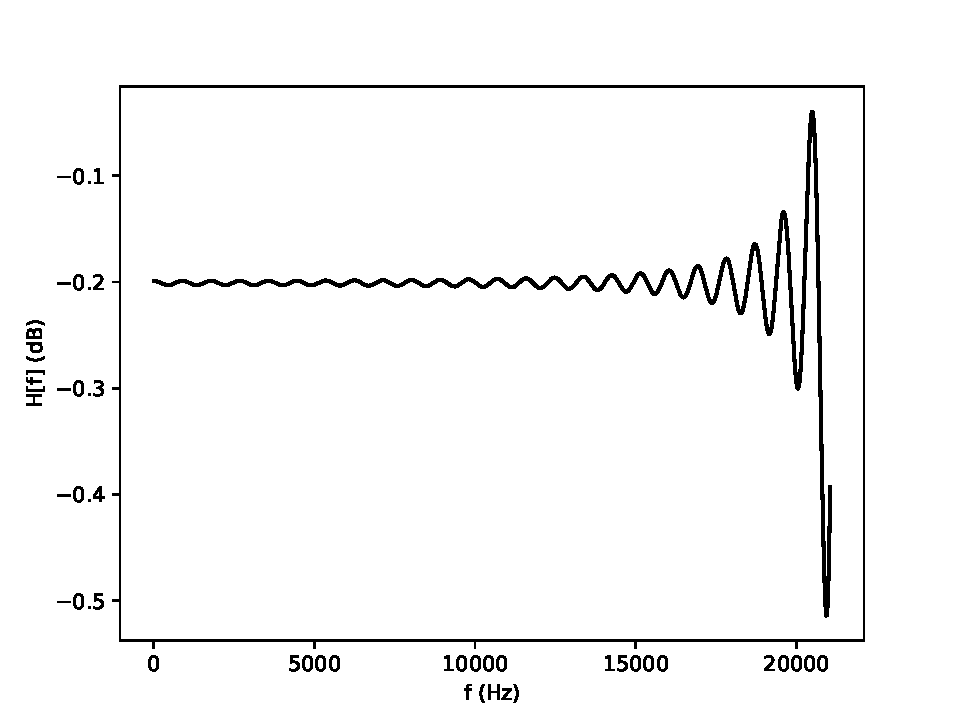
\includegraphics[scale=0.5]{fig/nowindow.pdf}
    \caption{Resposta impulsiva do filtro final sem janelamento}
    \label{fig:impulsiva nowindow}
\end{figure}

Me parece que o janelamento retangular já foi suficiente para resultar em um filtro "liso". 

Janelá-lo por Hamming inclusive introduz uma pequena imperfeição nas frequências baixas:
\begin{figure}[H]
    \centering
    \begin{multicols}{2}
        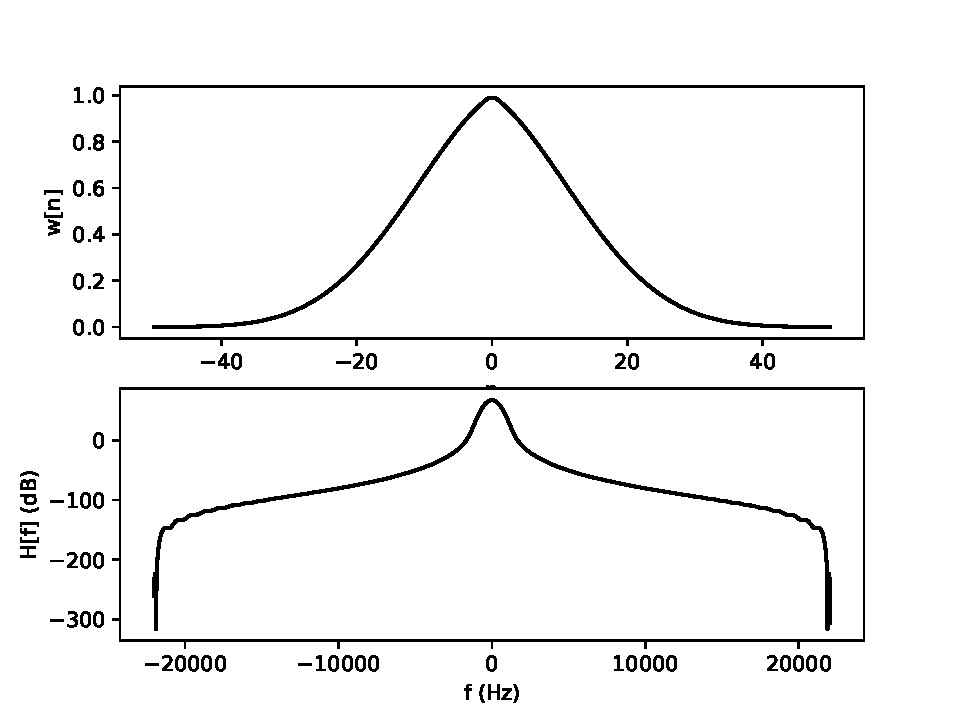
\includegraphics[scale=0.25]{fig/window.pdf}\\
        \small{Janela de Hamming}
        
        \columnbreak
        
        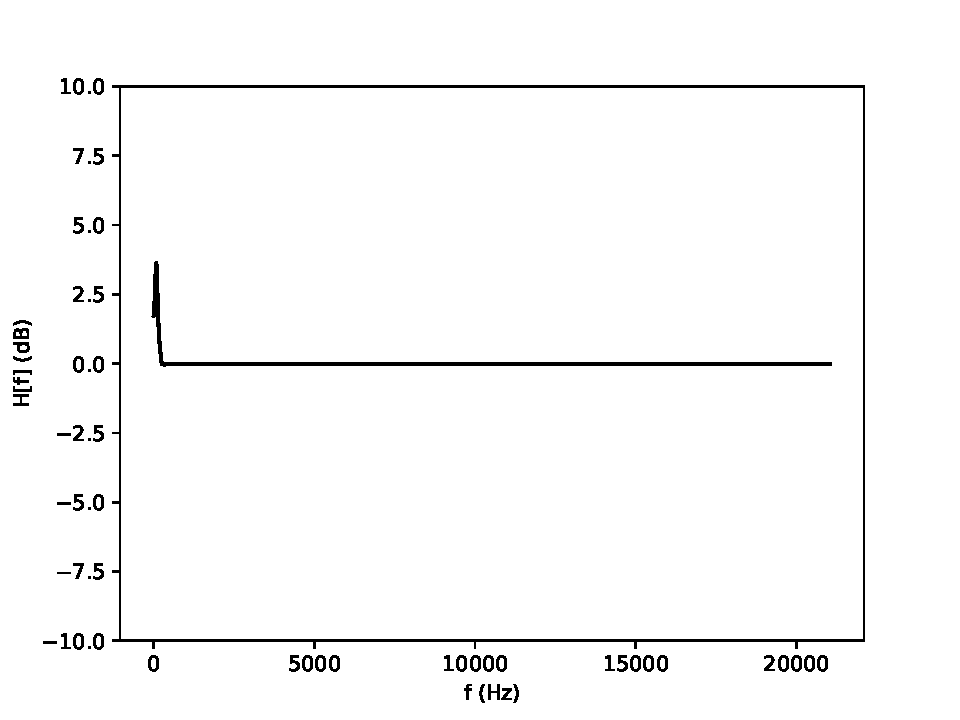
\includegraphics[scale=0.25]{fig/windowed.pdf}\\
        \small{Resposta impulsiva do filtro}
        
    \end{multicols}
    \caption{Resposta impulsiva do filtro final com janelamento Hamming}
    \label{fig:impulsiva window 1000}
\end{figure}
\end{multicols}

\begin{center}
    $\dots$
\end{center}

Nas seções seguintes, com filtros menores, apresento uma análise mais detalhada desse defeito.

Na prática, usar ou não o janelamento fez pouquíssima diferença nessa escala:
\begin{figure}[H]
    \minipage{0.5\textwidth}
        \centering
        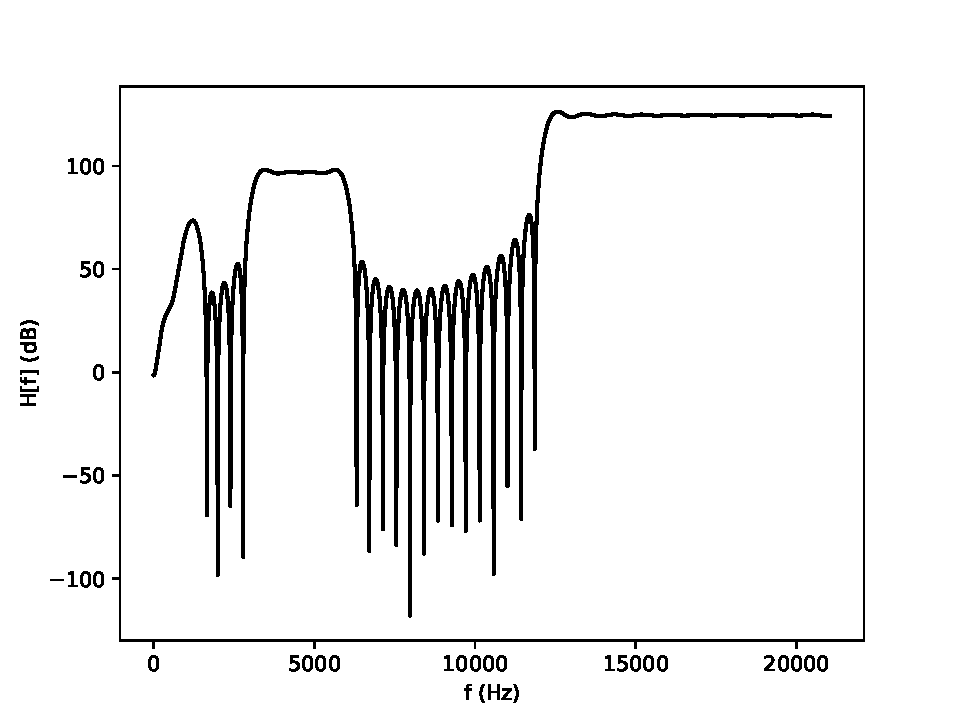
\includegraphics[scale=0.4]{fig/nowindow_stair.pdf}
    \endminipage
    \minipage{0.5\textwidth}
        \centering
        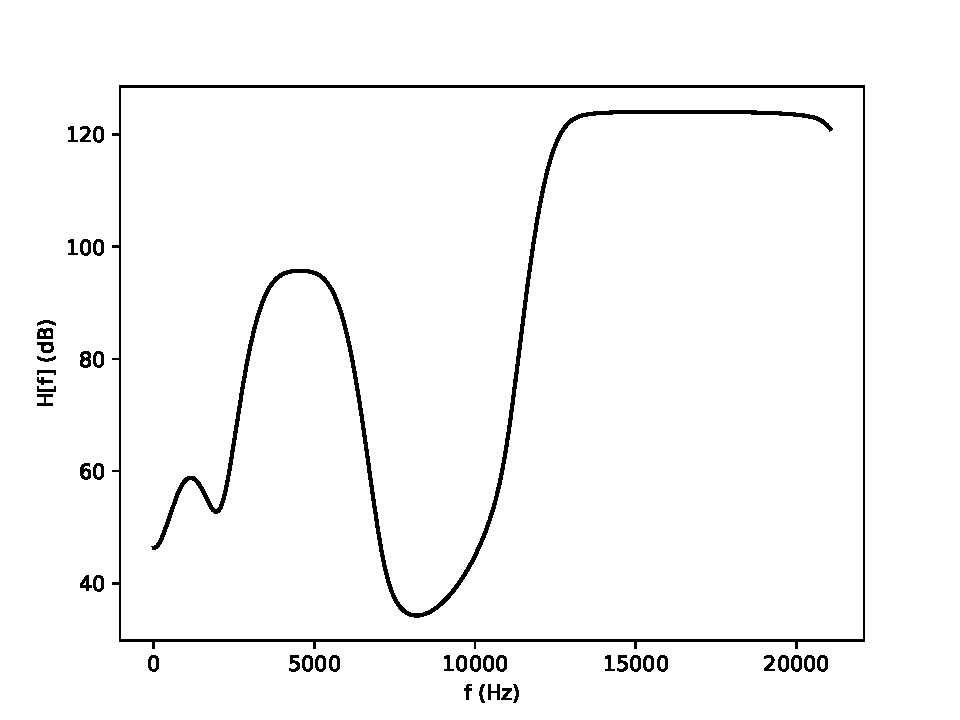
\includegraphics[scale=0.4]{fig/windowed_stair.pdf}
        \endminipage
    \begin{center}
        \caption{Resposta em frequência dos filtros sem e com janelamento}
        \small{(intensificando as bandas ímpares por $2^i$ e atenuando as pares)}
        \label{fig:stair window 1000}
    \end{center}
\end{figure}

\subsection{Filtros de tamanho 100}

\begin{multicols}{2}
Por problemas na implementação do host de áudio, o processamento em tempo real não funciona com filtros tão grandes, então re-desenhei filtros de tamanho 100 para poder testar na prática.

Assim como na seção \ref{1000}, foram desenhados 10 filtros cobrindo o espectro especificado, mas estes eram de largura $100$.

\begin{figure}[H]
    \centering
    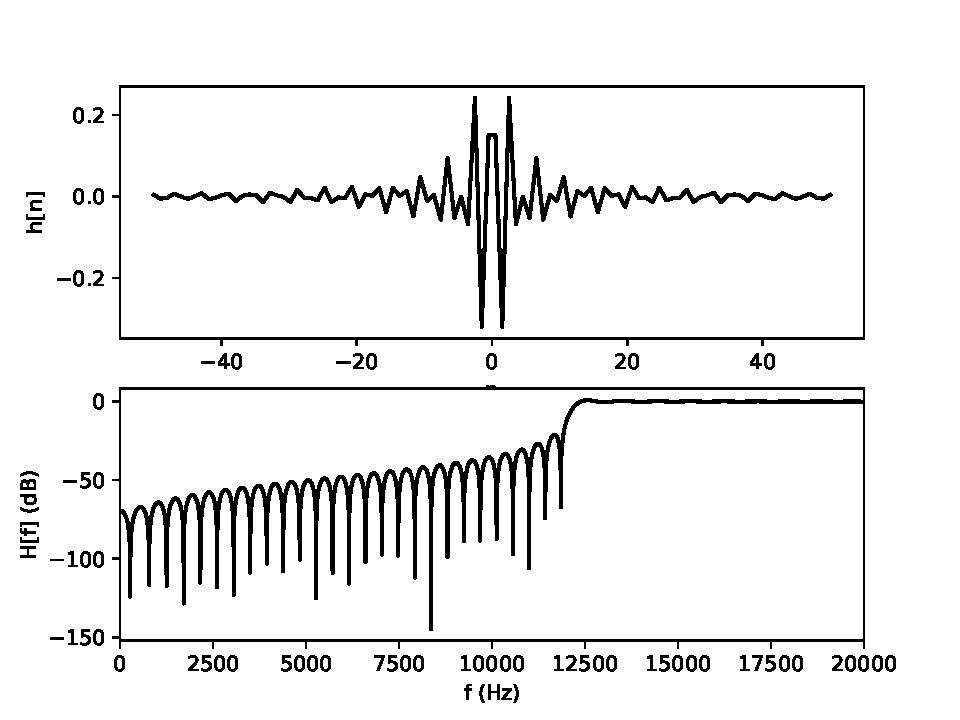
\includegraphics[scale=0.5]{fig/100/Hamming/filter9.pdf}
    \caption{Filtro da faixa 12k-22k}
    \label{fig:fnowindow}
\end{figure}

\begin{figure}[H]
    \centering
    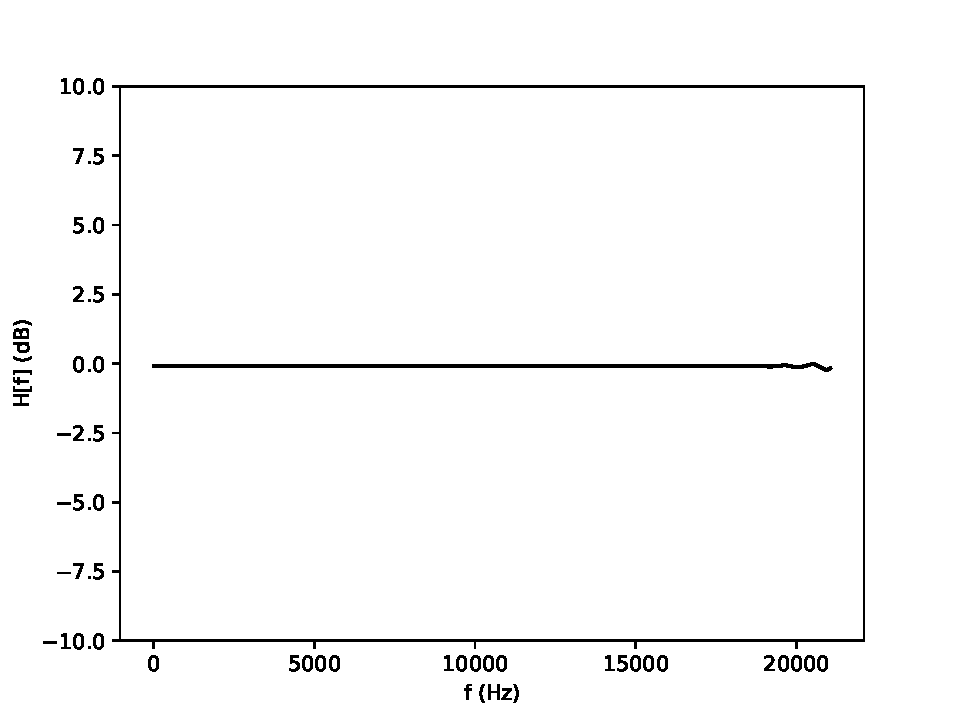
\includegraphics[scale=0.5]{fig/100/Hamming/nowindow.pdf}
    \caption{Resposta impulsiva do filtro final sem janelamento}
    \label{fig:imp resp total}
\end{figure}

Tanto no filtro individual como na resposta impulsiva do filtro final, temos imperfeições indesejáveis provindas da restrição dos filtros a $100$ amostras. Para minimizar esse problema, os filtros foram multiplicados por uma função de janelamento.

\end{multicols}

Com o janelamento por Hamming, reduzimos bastante as oscilações indesejáveis, mas a resposta para o filtro em um estado "neutro" super-representou as frequências baixas.

\begin{figure}[H]
    \centering
    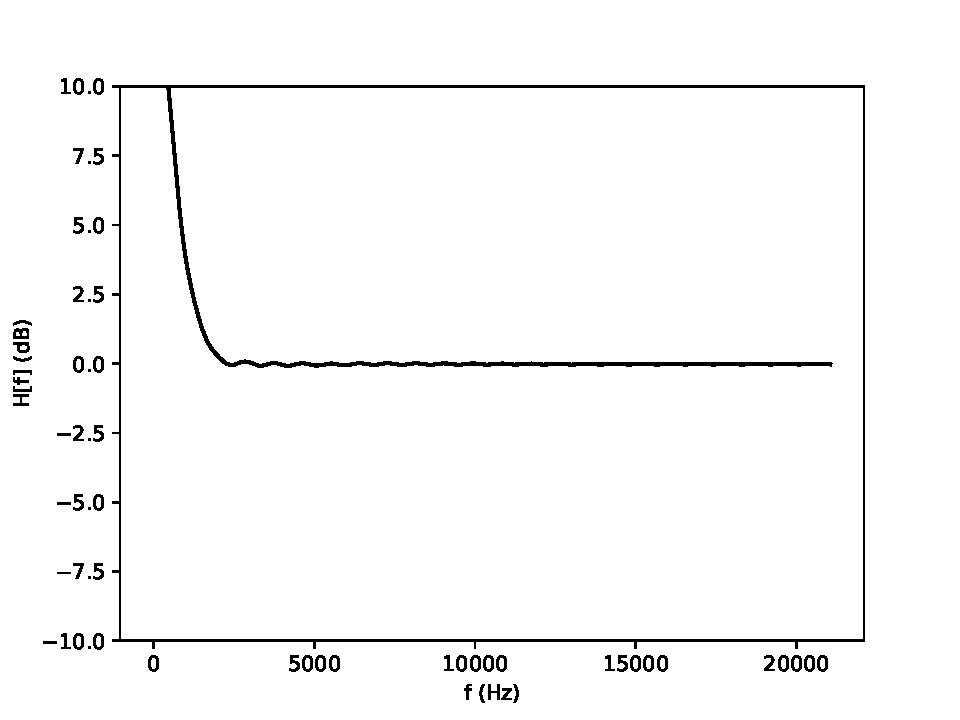
\includegraphics[scale=0.5]{fig/100/Hamming/windowed.pdf}
    \caption{Resposta impulsiva do filtro final com janelamento de Hamming}
    \label{fig:imp resp total hamm}
\end{figure}

Minha hipótese para explicar esse fenômeno estranho é que para filtros pequenos, os passa-faixas de baixas frequências são localizados demais para se diferenciarem. Por alguma razão, com janelamento retangular, alguma coisa compensa esse problema e deixa a resposta próxima ao desejado, mas com o janelamento essa intersecção/semelhança se evidencia mais.

\begin{figure}[H]
    \minipage{0.5\textwidth}
        \begin{center}
            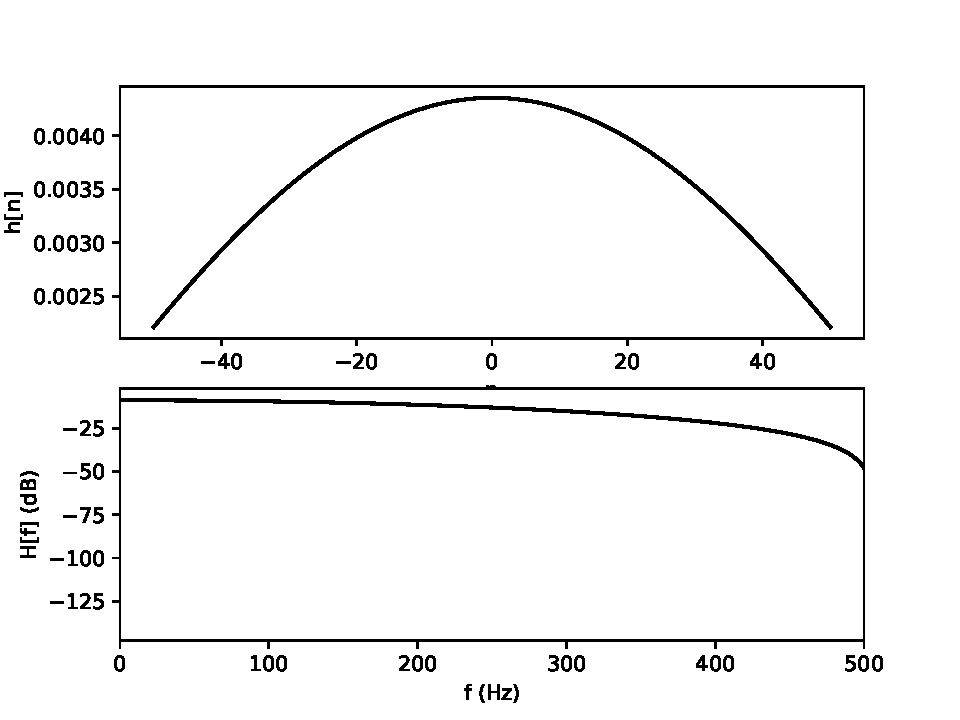
\includegraphics[scale=0.4]{fig/100/Hamming/filter2.pdf}\\
            \small{Filtro 96-192hz sem janelamento}
    
            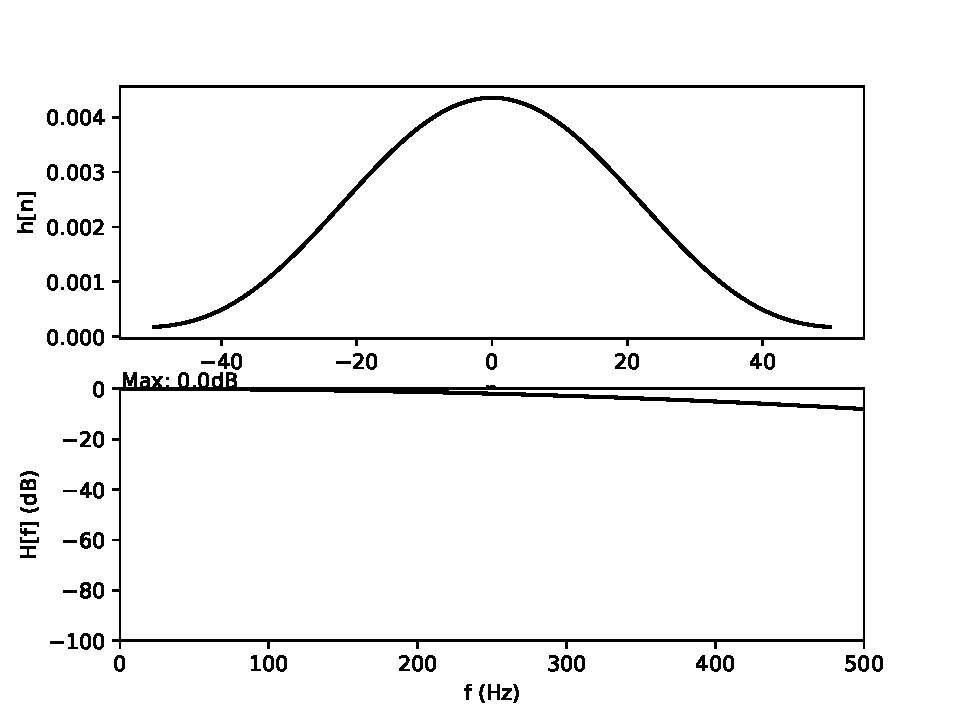
\includegraphics[scale=0.4]{fig/100/Hamming/windowfilter2.pdf}\\
            \small{Filtro 96-192hz com janelamento}
        \end{center}
    \endminipage
    \minipage{0.5\textwidth}
        \begin{center}
            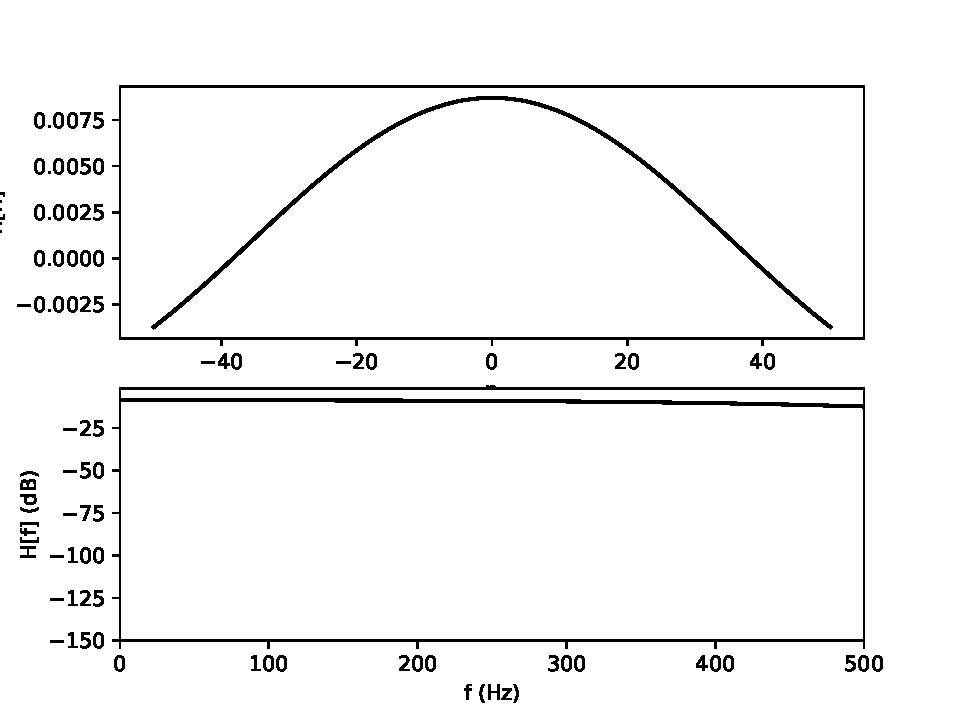
\includegraphics[scale=0.4]{fig/100/Hamming/filter3.pdf}\\
            \small{Filtro 192-384hz sem janelamento}
    
            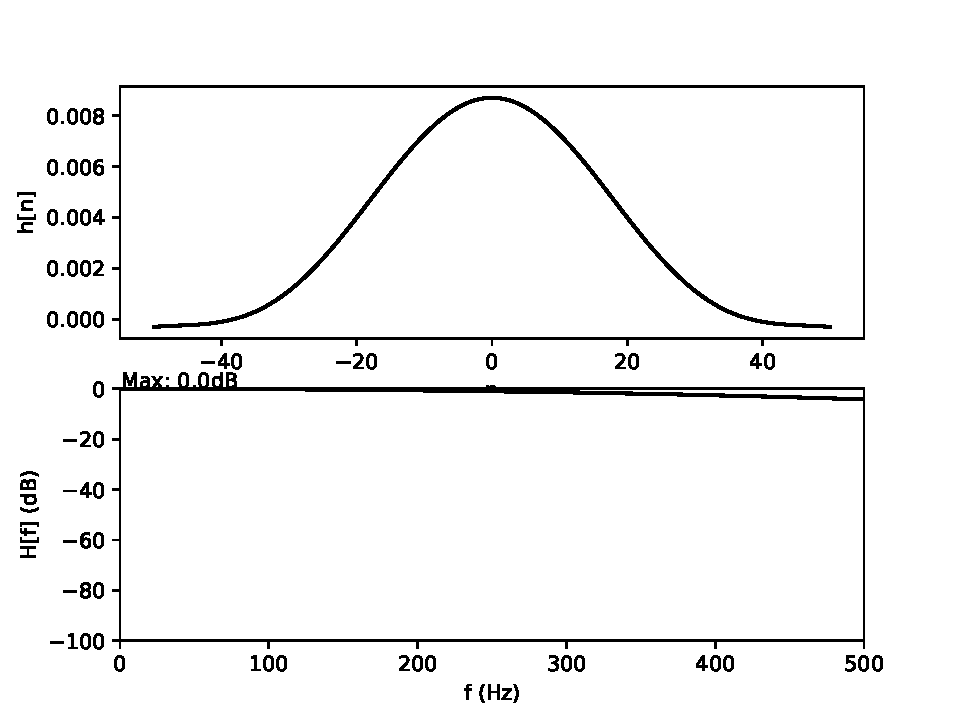
\includegraphics[scale=0.4]{fig/100/Hamming/windowfilter3.pdf}\\
            \small{Filtro 192-384hz com janelamento}
        \end{center}
    \endminipage
    \begin{center}
        \caption{Comparação dos filtros de tamanho 100 com e sem janelamento de Hamming}
        \label{fig:low 100}
    \end{center}
\end{figure}

\begin{figure}[H]
    \minipage{0.5\textwidth}
        \begin{center}
            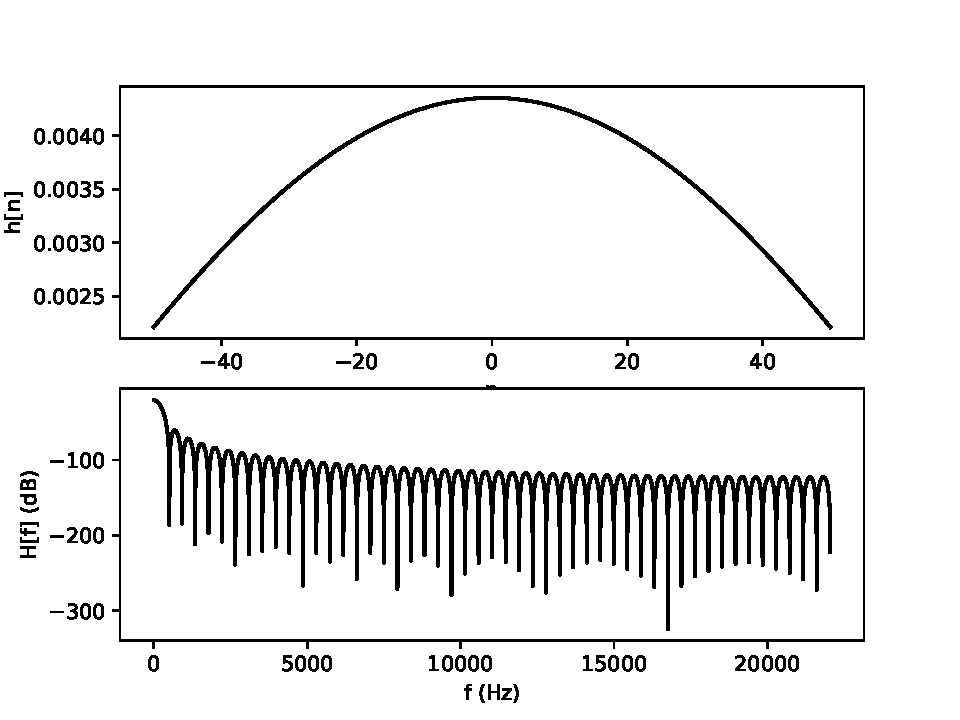
\includegraphics[scale=0.4]{fig/filter2.pdf}\\
            \small{Filtro 96-192hz sem janelamento}
    
            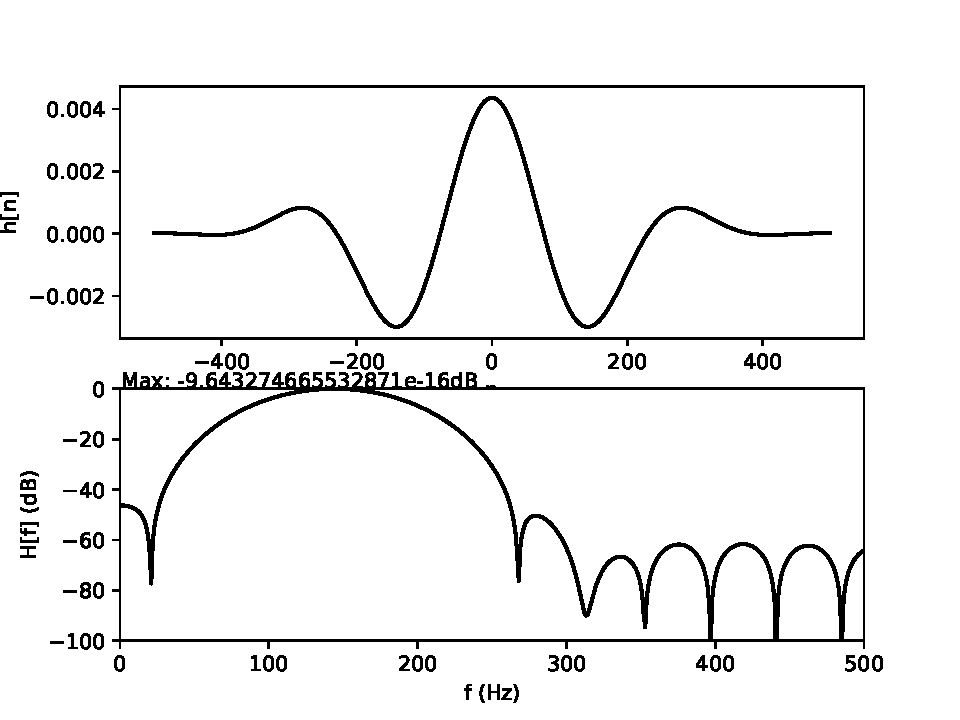
\includegraphics[scale=0.4]{fig/windowfilter2.pdf}\\
            \small{Filtro 96-192hz com janelamento}
        \end{center}
    \endminipage
    \minipage{0.5\textwidth}
        \begin{center}
            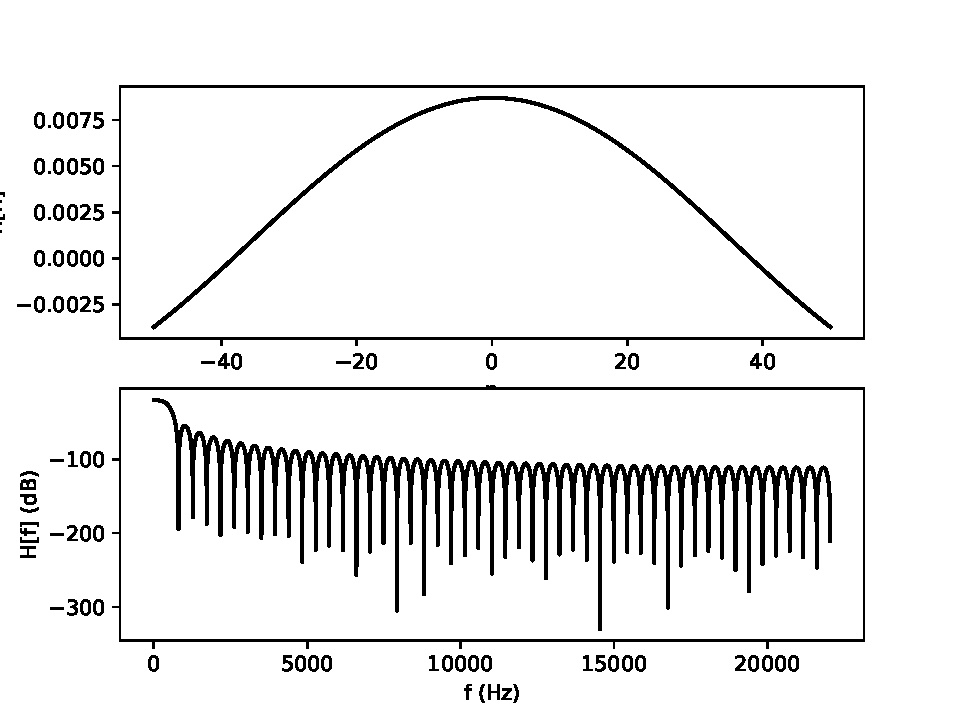
\includegraphics[scale=0.4]{fig/filter3.pdf}\\
            \small{Filtro 192-384hz sem janelamento}
    
            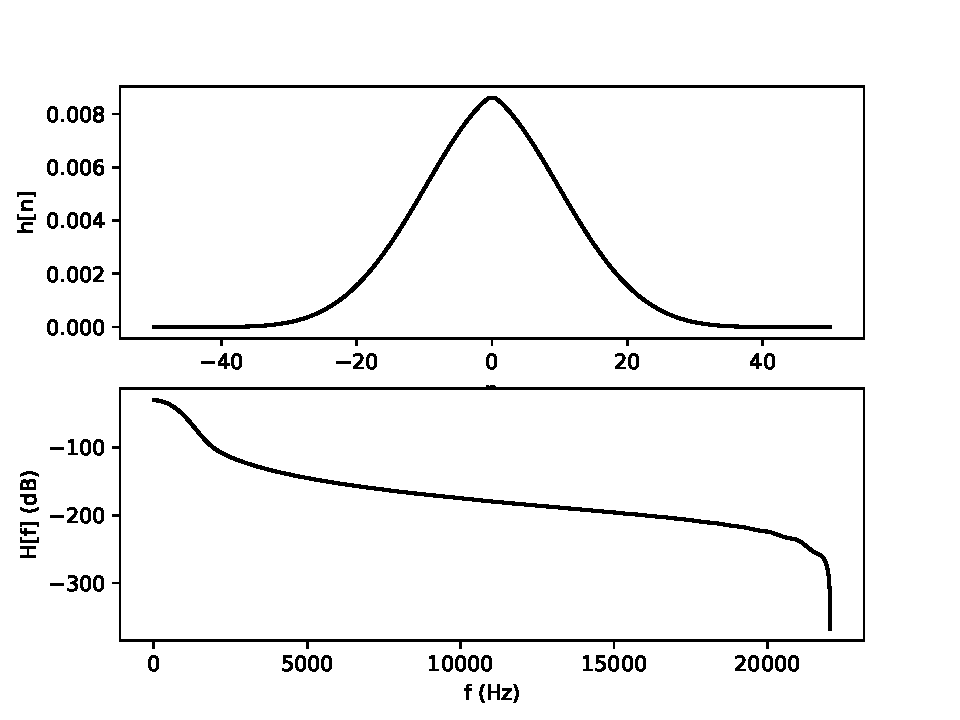
\includegraphics[scale=0.4]{fig/windowfilter3.pdf}\\
            \small{Filtro 192-384hz com janelamento}
        \end{center}
    \endminipage
    \begin{center}
        \caption{Comparação dos filtros de tamanho 1000 com e sem janelamento de Hamming}
        \label{fig:low 1000}
    \end{center}
\end{figure}